\documentclass[a4paper, 12pt]{article}

\usepackage[table,xcdraw]{xcolor}
\usepackage{enumerate}
\usepackage{graphicx}
\usepackage[T5]{fontenc}
\usepackage[utf8]{inputenc}
\usepackage[margin = 2cm]{geometry}
\usepackage{amsfonts, amsmath, amssymb}
\usepackage[none]{hyphenat}
\usepackage{fancyhdr}
\usepackage{float}
\usepackage{hyperref}
\usepackage{caption}
\usepackage[nottoc, notlot, notlof]{tocbibind}
% \usepackage{rotating}
% \usepackage{tikz}

\captionsetup[table]{skip=5pt}
\pagestyle{fancy}
\fancyhead[L]{Trường Đại học Khoa học Tự nhiên - ĐHQG TP.HCM}
\fancyhead[R]{Nhóm Just $4^{th}$}

\begin{document}
	\begin{titlepage}
		\begin{center}
			\vspace*{1cm}
			\Large\textbf{Báo cáo \#2\\Thiết kế hệ thống}\\
			
			\vfill
			\line(1,0){450}\\[4mm]
			\LARGE\textbf{\MakeUppercase{Dự án quản lý tạp chiếu phim}}\\[3mm]
			\Large{Nhập môn Công nghệ phần mềm (CSC13002)}\\[3mm]
			\Large{Nhóm Just $4^{th}$}
			\line(1,0){430}\\
			\vfill
			
			\vfill
			TP Hồ Chí Minh, ngày 07/11/2020
		\end{center}
	\end{titlepage}
	
	\tableofcontents
	\thispagestyle{empty}
	\clearpage
	
	\section{Thông tin nhóm}
	\label{sec:info}
	\begin{enumerate}
		\item \textbf{Đường link GitHub}: \url{https://github.com/baolongnguyenmac/CinemaManagementSystem}
		\item \textbf{Đường link Trello}: \url{https://trello.com/b/uymvzWAR/báo-cáo-thiết-kế-hệ-thống}
		\item \textbf{Danh sách thành viên}
		\begin{table}[H]
			\begin{center}
				\begin{tabular}{|c|c|l|c|c|}
					\hline
					STT & MSSV     & \multicolumn{1}{c|}{Họ tên} & Email                         & SĐT        \\ \hline
					1   & 18120201 & Nguyễn Bảo Long             & 18120201@student.hcmus.edu.vn & 0919070940 \\ \hline
					2   & 18120211 & Võ Thế Minh                 & 18120211@student.hcmus.edu.vn & 0981850699 \\ \hline
					3   & 18120227 & Phạm Văn Minh Phương        & 18120227@student.hcmus.edu.vn & 0343049359 \\ \hline
					4   & 18120210 & Phạm Tống Bình Minh         & 18120210@student.hcmus.edu.vn & 0971877781 \\ \hline
					5   & 18120264 & Nguyễn Duy Vũ               & 18120264@student.hcmus.edu.vn & 0911572108 \\ \hline
				\end{tabular}
				\caption{Bảng danh sách thành viên nhóm}
			\end{center}
		\end{table}
	\end{enumerate}
	\clearpage
	
	\section{Lịch sử cập nhật}
	\label{sec:history}
	\begin{table}[h]
		\begin{center}
			\begin{tabular}{|c|c|c|l|l|}
				\hline
				STT &Ngày cập nhật &Phiên bản &\multicolumn{1}{c|}{Mô tả chi tiết} &\multicolumn{1}{c|}{Tác giả} \\ \hline
				% 1 &22/10/2020 &1.0 &\begin{tabular}[c]{@{}l@{}}- Nhận diện thành viên nhóm\\ - Mô tả bài toán\\ - Yêu cầu hệ thống\\ - Xác định stakeholder\\ - Xác định actor\end{tabular} &\begin{tabular}[c]{@{}l@{}}Phạm Tống Bình Minh\\ Nguyễn Bảo Long\\ Nguyễn Duy Vũ\end{tabular} \\ \hline
				% 2 &25/10/2020 &1.1 &\begin{tabular}[c]{@{}l@{}}- Đặc tả use case\\ - Vẽ biểu đồ use case\\- Vẽ biểu đồ tuần tự\\ - Lên kế hoạch làm việc\end{tabular} &\begin{tabular}[c]{@{}l@{}}Phạm Tống Bình Minh\\ Nguyễn Duy Vũ\\Nguyễn Bảo Long \\ Võ Thế Minh\end{tabular} \\ \hline
				% 3 &25/10/2020 &1.2 &\begin{tabular}[c]{@{}l@{}}- Đặc tả giao diện người dùng\\ - Lên kế hoạch làm việc\end{tabular} &\begin{tabular}[c]{@{}l@{}}Nguyễn Bảo Long \\ Võ Thế Minh \\ Phạm Văn Minh Phương\end{tabular} \\ \hline
				% 4 &30/10/2020 &1.3 &- Đặc tả giao diện người dùng &Phạm Văn Minh Phương \\ \hline
				% 5 &31/10/2020 &1.5 &- Phân tích đóng góp cá nhân &Phạm Văn Minh Phương \\ \hline
			\end{tabular}
			\caption{Bảng lịch sử cập nhật các phiên bản của báo cáo yêu cầu}
		\end{center}
	\end{table}
	\clearpage
	
	\section{Phân tích đóng góp cá nhân}
	\label{sec:analys}
	\begin{table}[H]
		\begin{center}
			\begin{tabular}{|c|l|l|c|}
				\hline
				STT & \multicolumn{1}{c|}{Họ tên} & \multicolumn{1}{c|}{Công việc tham gia}                                                & Phần trăm đóng góp \\ \hline
				% 1 & Nguyễn Bảo Long      & \begin{tabular}[c]{@{}l@{}}- Mô tả bài toán\\ - Mô tả yêu cầu hệ thống\\ - Vẽ biểu đồ tuần tự\end{tabular}              & 20\% \\ \hline
				% 2 & Phạm Văn Minh Phương & \begin{tabular}[c]{@{}l@{}}- Nhận diện thành viên\\ - Đặc tả giao diện người dùng\end{tabular}                          & 20\% \\ \hline
				% 3   & Võ Thế Minh                 & \begin{tabular}[c]{@{}l@{}}- Vẽ biểu đồ tuần tự\\ - Lên kế hoạch làm việc\end{tabular} & 20\%               \\ \hline
				% 4 & Phạm Tống Bình Minh  & \begin{tabular}[c]{@{}l@{}}- Đặc tả use case\\ - Vẽ ma trận truy vết\\ - Vẽ biểu đồ use case\end{tabular}               & 20\% \\ \hline
				% 5 & Nguyễn Duy Vũ        & \begin{tabular}[c]{@{}l@{}}- Lên danh sách actor, stakeholder\\ - Đặc tả use case \\ - Vẽ ma trận truy vết\end{tabular} & 20\% \\ \hline
			\end{tabular}
			\caption{Bảng phân tích đóng góp cá nhân}
		\end{center}
	\end{table}
	\clearpage
	
	\section{Thiết kế kiến trúc và hệ thống}
	
	\subsection{Kiến trúc hệ thống}
	\begin{figure}[H]
		\begin{center}
			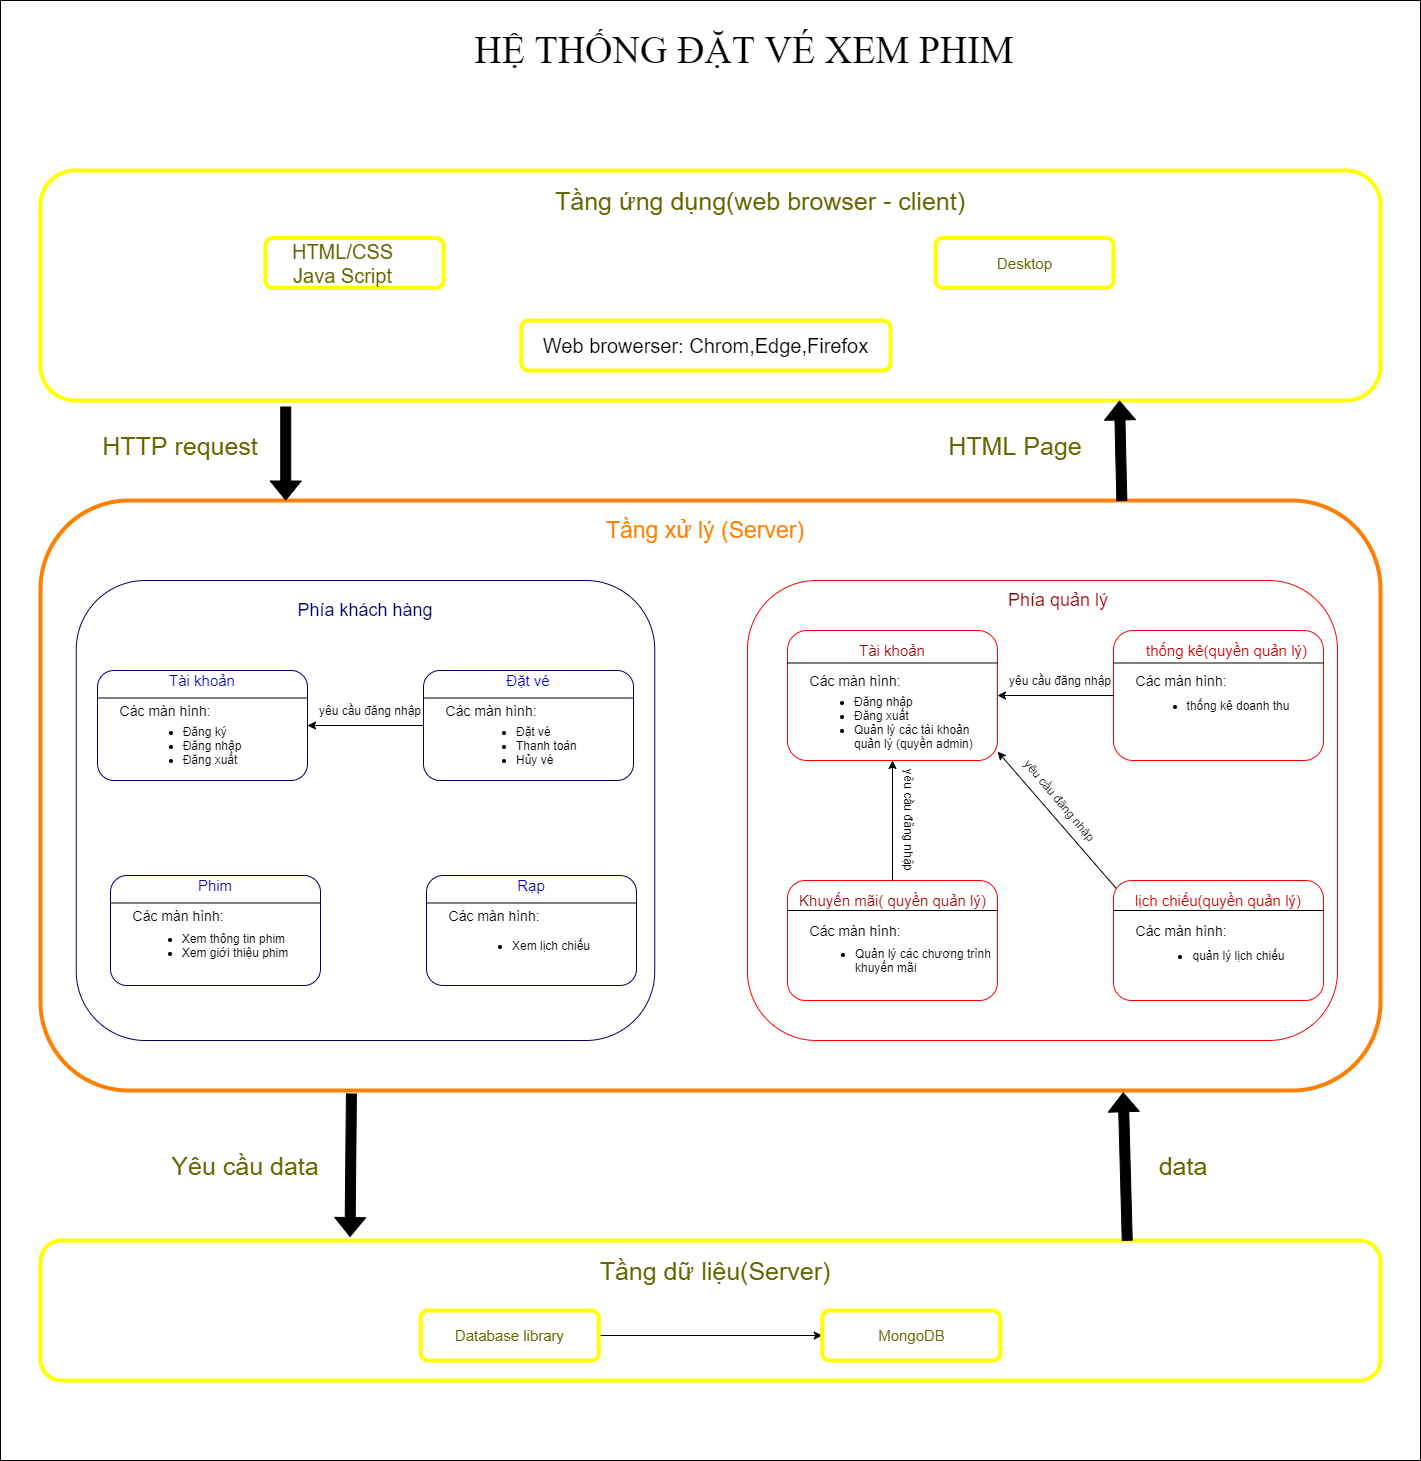
\includegraphics[scale = 0.25]{image/4.1.png}
			\caption{Kiến trúc tổng thể hệ thống}
		\end{center}
	\end{figure}
	%text description
	Hệ thống đặt vé xem phim sử dụng kiến trúc Client - Server :
	\begin{itemize}
		\item Ở phía Client sử dụng Web Browser được mở từ các thiết bị (PC, Laptop, SmartPhone,...) để truy cập vào trang web.
		\item Ở phía Server sẽ xử lý các yêu cầu (HTTP request) được gửi từ Client thông qua các module và trả về các page HTML hiện thị trên Web Browser.Ở hệ thống này nhóm dùng node.js để xây dựng hệ thống.
		\item Quá trình xử lý ở Server có thể yêu cầu truy xuất cơ sở dữ liệu (CRUD) được lưu ở hệ quản trị cơ sở dữ liệu. Ở hệ thống này nhóm dùng hệ quản trị cơ sở dữ liệu MySQL.
	\end{itemize}
	
	\subsection{Nhận diện hệ thống con}
	\begin{figure}[H]
		\begin{center}
			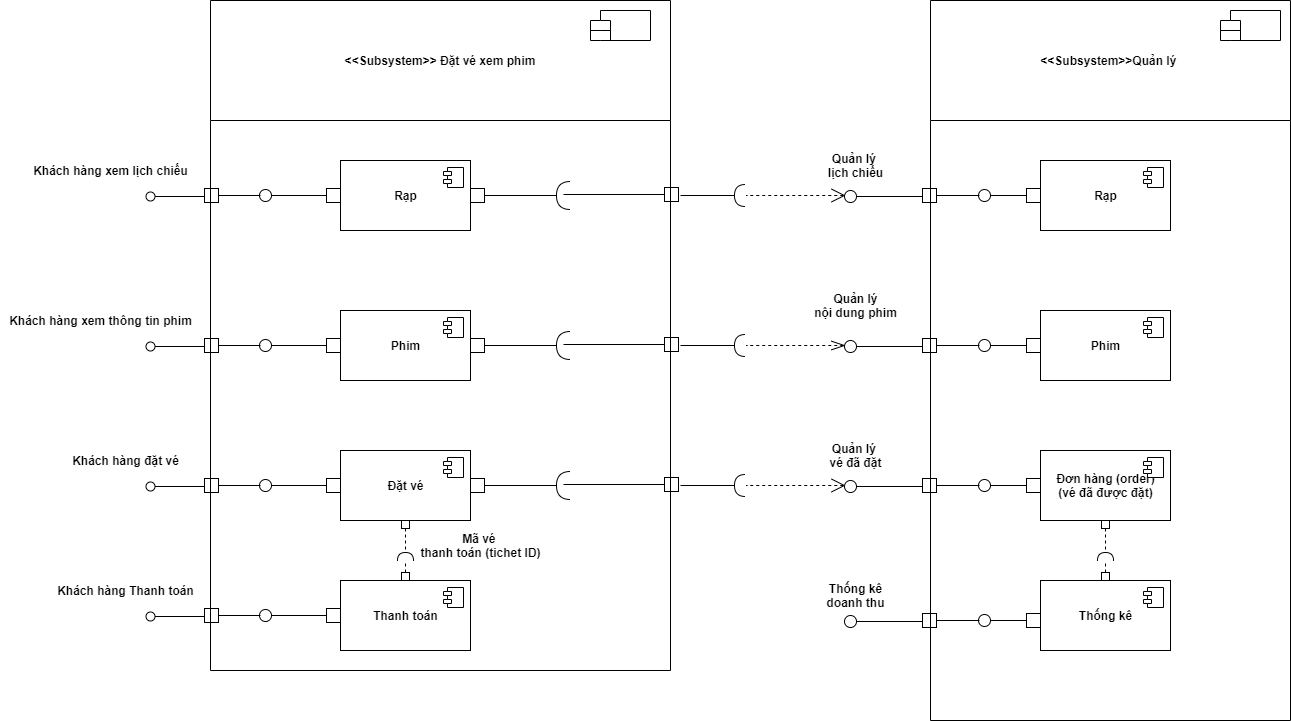
\includegraphics[scale = 0.35]{image/4.2.png}
			\caption{Component Diagram}
		\end{center}
	\end{figure}
	%text description
	Hệ thống đặt vé xem phim có 2 hệ thống con :
	\begin{itemize}
		\item Hệ thống con đặt vé xem phim với các component:
		\begin{enumerate}
			\item Rạp : cung cấp chức năng xem lịch chiếu. 
			\item Phim : cung cấp chức năng xem thông tin phim.
			\item Đặt vé : cung cấp chức năng đặt vé.
			\item Thanh Toán : cung cấp chức năng thanh toán.
		\end{enumerate}
		\item Hệ thống con quản lý với các component
		\begin{enumerate}
			\item Rạp : cung cấp chức năng xem lịch chiếu.
			\item Phim: cung cấp chức năng xem lịch chiếu.
			\item Đơn hàng:cung cấp chức năng xem quản lý vé đã đặt.
			\item Thống kê: cung cấp chức năng thống kê doanh thu.
		\end{enumerate}
	\end{itemize}
	\subsection{Ánh xạ các phần của hệ thống với phần cứng}
	\begin{figure}[H]
		\begin{center}
			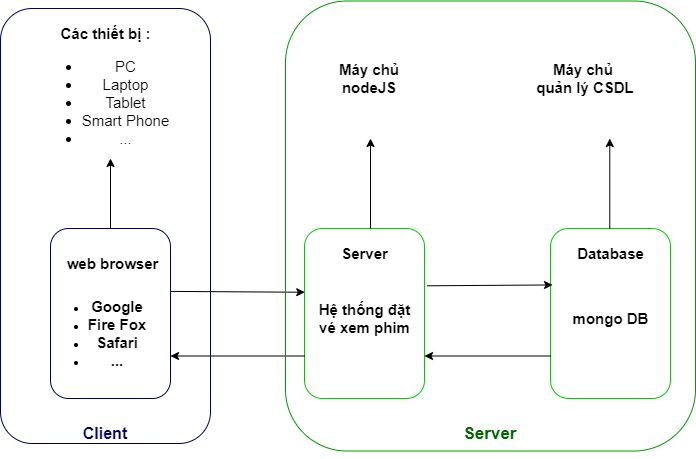
\includegraphics[scale = 0.5]{image/4.3.png}
			\caption{Ánh xạ hệ thống tới phần cứng}
		\end{center}
	\end{figure}
	%text description
	Hệ thống đặt vé xem phim sử dụng mô hình Client - Server thì có các phần cứng :
	\begin{itemize}
		\item Ở phía Client sẽ sử dụng các thiết bị như Laptop, PC, SmartPhone , Table, ... để truy cập vào hệ thống thông qua Web Browser như Google, Safari, FireFox ...
		\item Ở phía Server sẽ sử dụng các máy chủ để chạy Server và hệ quản trị cơ sở dữ liệu.
	\end{itemize}
	\subsection{Lưu trữ dữ liệu lâu dài}
	\begin{figure}[H]
		\begin{center}
			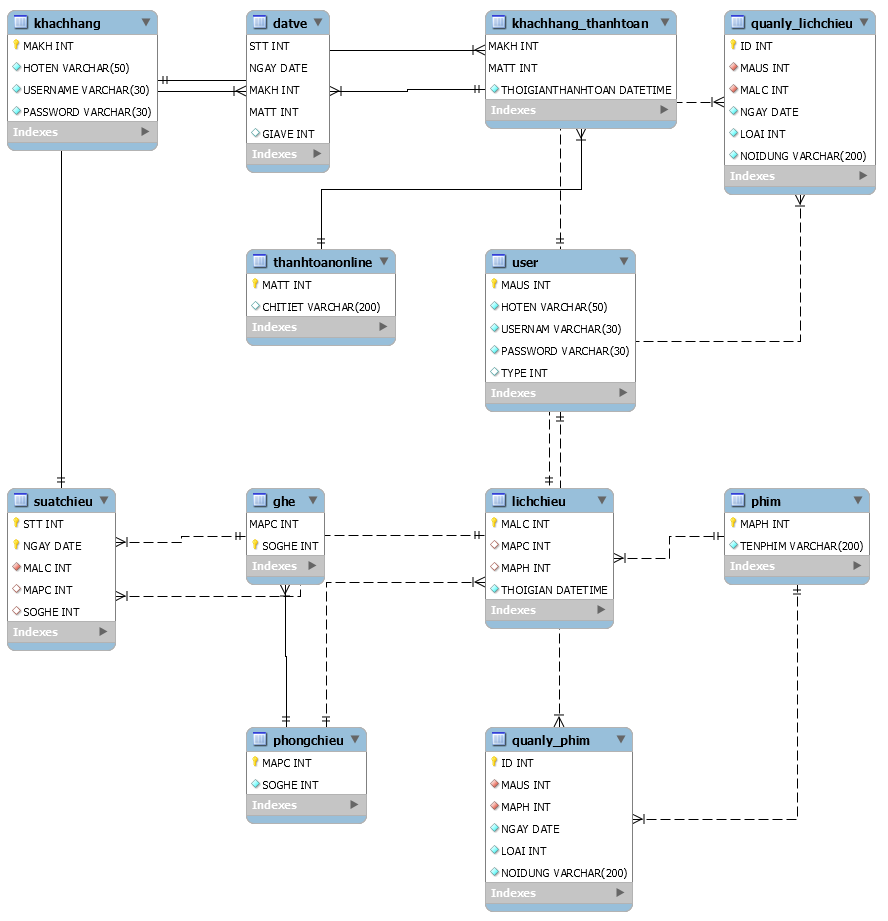
\includegraphics[scale = 0.25]{image/4.4.png}
			\caption{Database Diagram}
		\end{center}
	\end{figure}
	%text description
	Hệ thống đặt vé xem phim sử dụng MySQL làm hệ quản trị CSDL với các Table:
	\begin{itemize}
		\item PHIM: lưu thông tin Phim.
		\item PHONGCHIEU: lưu thông tin phòng chiếu.
		\item GHE: lưu thông tin về ghế trong PHONGCHIEU.
		\item LICHCHIEU: lưu thông tin lịch chiếu.
		\item SUATCHIEU: lưu thông tin suất chiếu.
		\item DATVE: lưu thông tin đặt vé của khách hàng.
		\item KHACHHANG\_THANHTOAN: lưu thông tin về thanh toán của vé đã đặt.
		\item THANHTOANONLINE: lưu thông tin về thanh toán online cho 1 đơn hàng(đặt vé) thông qua KHACHHANG\_THANHTOAN.
		\item KHACHHANG: lưu thông tin về khách hàng
		\item USER: lưu thông tin về Quản lý và Admin
		\item QUANLIPHIM: lưu lịch sử của việc quản lý (thêm, xóa, sửa) phim.
		\item QUANLILICHCHIEU: lưu lịch sử của việc quản lý (thêm, xóa, sửa) lịch chiếu.
	\end{itemize}	
<<<<<<< HEAD
\subsection{Giao thức mạng}

\subsection{Luồng điều khiển (Global Control Flow)}

\subsection{Yêu cầu phần cứng}

\clearpage

\section{Biểu đồ lớp}

\subsection{Biểu đồ lớp}
\begin{figure}[H]
\centering
	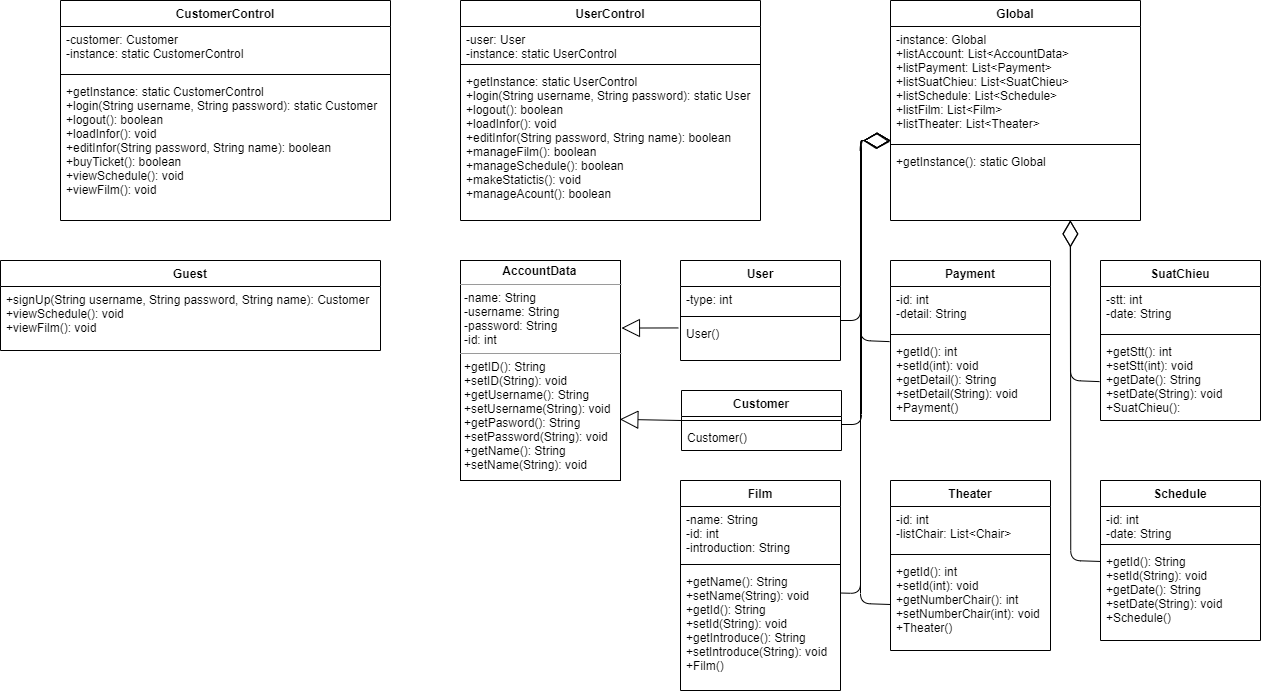
\includegraphics[scale=0.37]{image/5.0.png}
	\caption{Class Diagram}
\end{figure}

\subsection{Đặc tả các lớp}

\subsubsection{Lớp AccountData}
\begin{table}[h]
\centering
	\begin{tabular}{|l|l|l|l|l|}
	\hline
	STT & Tên thuộc tính & Loại   & Ràng buộc & Ý nghĩa             \\ \hline
	1   & name           & private &           & Tên người dùng      \\ \hline
	2   & username       & private &           & Tài khoản đăng nhập \\ \hline
	3   & password       & private &           & Mật khẩu đăng nhập  \\ \hline
	4   & id             & private &           & Định danh tài khoản \\ \hline
	\end{tabular}
\end{table}
\begin{table}[H]
\centering
		\begin{tabular}{|l|l|l|l|l|}
		\hline
		STT & Tên phương thức          & Loại   & Ràng buộc & Ý nghĩa                                                                           \\ \hline
		1   & Các phương thức get, set & public &           & \begin{tabular}[c]{@{}l@{}}Lấy hoặc gán giá trị cho\\ các thuộc tính\end{tabular} \\ \hline
		\end{tabular}
\end{table}

\subsubsection{Lớp User-Kế thừa lớp AccountData}
\begin{table}[H]
\centering
	\begin{tabular}{|l|l|l|l|l|}
		\hline
		STT & Tên thuộc tính & Loại    & Ràng buộc & Ý nghĩa             \\ \hline
		1   & type           & private &           & Loại User(Quản lí, Admin)      \\ \hline
		\end{tabular}
	\end{table}
\begin{table}[H]
\centering
	\begin{tabular}{|l|l|l|l|l|}
	\hline
	STT & Tên phương thức          & Loại   & Ràng buộc & Ý nghĩa                                                                           \\ \hline
	1   & User() 				   & public &           & Khởi tạo đối tượng user \\ \hline
	\end{tabular}
\end{table}

\subsubsection{Lớp Customer-Kế thừa lớp AccountData}
\begin{table}[H]
\centering
	\begin{tabular}{|l|l|l|l|l|}
		\hline
		STT & Tên phương thức          & Loại   & Ràng buộc & Ý nghĩa                                                                           \\ \hline
		1   & Customer() 				   & public &           & Khởi tạo đối tượng user \\ \hline
	\end{tabular}
\end{table}

\subsubsection{Lớp Payment}
\begin{table}[H]
\centering
\begin{tabular}{|l|l|l|l|l|}
\hline
STT & Tên thuộc tính & Loại    & Ràng buộc & Ý nghĩa                  \\ \hline
1   & id             & private &           & Định danh một thanh toán \\ \hline
2   & detail         & private &           & Chi tiết một thanh toán  \\ \hline
\end{tabular}
\end{table}
\begin{table}[H]
\centering
\begin{tabular}{|l|l|l|l|l|}
\hline
STT & Tên thuộc tính & Loại    & Ràng buộc & Ý nghĩa                  \\ \hline
1   & id             & private &           & Định danh một thanh toán \\ \hline
2   & detail         & private &           & Chi tiết một thanh toán  \\ \hline
\end{tabular}
\end{table}

\subsubsection{Lớp SuatChieu}
\begin{table}[H]
\centering
\begin{tabular}{|l|l|l|l|l|}
\hline
STT & Tên thuộc tính & Loại    & Ràng buộc & Ý nghĩa                             \\ \hline
1   & stt            & private &           & Số thứ tự của suất chiếu trong ngày \\ \hline
2   & date           & private &           & Ngày khởi tạo suất chiếu            \\ \hline
\end{tabular}
\end{table}
\begin{table}[H]
\centering
\begin{tabular}{|l|l|l|l|l|}
\hline
STT & Tên phương thức          & Loại   & Ràng buộc & Ý nghĩa                             \\ \hline
1   & Các phương thức get, set & public &           & Lấy hoặc gán giá trị cho thuộc tính \\ \hline
2   & Payment                  & public &           & Khởi tạo một đối tượng thanh toán   \\ \hline
\end{tabular}
\end{table}

\subsubsection{Lớp Film}
\begin{table}[H]
\centering
\begin{tabular}{|l|l|l|l|l|}
\hline
STT & Tên thuộc tính & Loại    & Ràng buộc & Ý nghĩa                	\\ \hline
1   & name           & private &           & Tên phim 					\\ \hline
2   & id             & private &           & Định danh phim           	\\ \hline
3   & introduction   & private &           & Giới thiệu phim          	\\ \hline
\end{tabular}
\end{table}
\begin{table}[H]
\centering
\begin{tabular}{|l|l|l|l|l|}
\hline
STT & Tên phương thức          & Loại   & Ràng buộc & Ý nghĩa                                 \\ \hline
1   & Các phương thức get, set & public &           & Lấy hoặc gán giá trị cho các thuộc tính \\ \hline
2   & Film                     & public &           & Khởi tạo một đối tượng phim             \\ \hline
\end{tabular}
\end{table}

\subsubsection{Lớp Theater}
\begin{table}[H]
\centering
\begin{tabular}{|l|l|l|l|l|}
\hline
STT & Tên thuộc tính & Loại    & Ràng buộc & Ý nghĩa                    \\ \hline
1   & id           	 & private &           & Định danh phim phòng chiếu \\ \hline
2   & listChair      & private &           & Danh sách ghế              \\ \hline
\end{tabular}
\end{table}
\begin{table}[H]
\centering
\begin{tabular}{|l|l|l|l|l|}
\hline
STT & Tên phương thức          & Loại   & Ràng buộc & Ý nghĩa                                 \\ \hline
1   & Các phương thức get, set & public &           & Lấy hoặc gán giá trị cho các thuộc tính \\ \hline
2   & Theatẻ                   & public &           & Khởi tạo một đối tượng phòng chiếu      \\ \hline
\end{tabular}
\end{table}

\subsubsection{Lớp Schedule}
\begin{table}[H]
\centering
\begin{tabular}{|l|l|l|l|l|}
\hline
STT & Tên thuộc tính           & Loại   & Ràng buộc & Ý nghĩa                                 \\ \hline
1   & Các phương thức get, set & public &           & Lấy hoặc gán giá trị cho các thuộc tính \\ \hline
2   & Schedule                 & public &           & Khởi tạo một đối tượng lịch chiếu       \\ \hline
\end{tabular}
\end{table}

\begin{table}[H]
\centering
\begin{tabular}{|l|l|l|l|l|}
\hline
STT & Tên thuộc tính  & Loại    & Ràng buộc & Ý nghĩa                  \\ \hline
1   & id              & private &           & Định danh một lịch chiếu \\ \hline
2   & date            & private &           & Ngày khởi tạo lịch chiếu \\ \hline
\end{tabular}
\end{table}

\subsubsection{Lớp Global}
\begin{table}[H]
\centering
\begin{tabular}{|l|l|l|l|l|}
\hline
STT & Tên thuộc tinh  & Loại     & Ràng buộc & Ý nghĩa                                                                                                      \\ \hline
1   & instance        & priavate &           & \begin{tabular}[c]{@{}l@{}}Đối tượng Global duy nhất được\\ tạo để quản lí dữ liệu toàn cục\end{tabular} \\ \hline
2   & listAccount     & public   &           & Quản lí danh sách các AccountData                                                                            \\ \hline
3   & listPayment     & public   &           & Quản lí danh sách các Payment                                                                                \\ \hline
4   & listSuatChieu   & public   &           & Quản lí danh sách các Suất chiếu                                                                             \\ \hline
5   & listSchedule    & public   &           & Quản lí danh sách các lịch chiếu                                                                             \\ \hline
6   & listFilm        & public   &           & Quản lí danh sách các phim                                                                                   \\ \hline
7   & listTheater     & public   &           & Quản lí danh sách các phòng chiếu                                                                            \\ \hline
\end{tabular}
\end{table}

\begin{table}[H]
\centering
\begin{tabular}{|l|l|l|l|l|}
\hline
STT & Tên phương thức & Loại    & Ràng buộc & Ý nghĩa                                                                                                      \\ \hline
1   & instance        & private &           & \begin{tabular}[c]{@{}l@{}}Đối tượng duy nhất của Global được\\ tạo để quản lí dữ liệu toàn cục\end{tabular} \\ \hline
\end{tabular}
\end{table}

\subsubsection{Lớp UserControl}
\begin{table}[H]
\centering
\begin{tabular}{|l|l|l|l|l|}
\hline
STT & Tên thuộc tính & Loại    & Ràng buộc & Ý nghĩa                                           \\ \hline
1   & user           & private &           & Dữ liệu user của UserControl                      \\ \hline
2   & instance       & private &           & Đối tượng user duy nhất được tạo ra khi đăng nhập \\ \hline
\end{tabular}
\end{table}
\begin{table}[H]
\centering
\begin{tabular}{|l|l|l|l|l|}
\hline
STT & Tên phương thức & Loại   & Ràng buộc & Ý nghĩa                                              \\ \hline
1   & getInstance     & public &           & Truy xuất đối tượng UserControl duy nhất             \\ \hline
2   & login           & public &           & Đăng nhập, nếu đúng trả về một User(quản lí)         \\ \hline
3   & logout          & public &           & Đăng xuất tài khoản(quản lí)                         \\ \hline
4   & loadInfor       & public &           & Xem thông tin cá nhân(quản lí)                       \\ \hline
5   & manageFilm      & public &           & Quản lí phim(thêm, xóa, sửa)(quản lí)                \\ \hline
6   & manageSchedule  & public &           & Quản lí lịch chiếu(thêm, xóa, sửa)(quản lí)          \\ \hline
7   & makeStatic      & public &           & Thống kê doanh thu(admin)                            \\ \hline
8   & manageAccount   & public &           & Quản lí các tài khoản quản lí(thêm, xóa, sửa)(admin) \\ \hline
\end{tabular}
\end{table}
\subsubsection{Lớp CustomerControl}
\begin{table}[H]
\centering
\begin{tabular}{|l|l|l|l|l|}
\hline
STT & Tên thuộc tính & Loại    & Ràng buộc & Ý nghĩa                                           \\ \hline
1   & user           & private &           & Dữ liệu user của UserControl                      \\ \hline
2   & instance       & private &           & Đối tượng user duy nhất được tạo ra khi đăng nhập \\ \hline
\end{tabular}
\end{table}

\begin{table}[H]
\centering
\begin{tabular}{|l|l|l|l|l|}
\hline
STT & Tên phương thức & Loại   & Ràng buộc & Ý nghĩa                                      \\ \hline
1   & getInstance     & public &           & Truy xuất đối tượng CustomerControl          \\ \hline
2   & login           & public &           & Đăng nhập, nếu chính xác trả về một Customer \\ \hline
3   & logout          & public &           & Đăng xuất, nếu đúng trả về true và ngược lại \\ \hline
4   & loadInfor       & public &           & Xem thông tin cá nhân                        \\ \hline
5   & editInfor       & public &           & Chỉnh sửa thông tin cá nhân                  \\ \hline
6   & buyTicket       & public &           & Mua vé                                       \\ \hline
\end{tabular}
\end{table}

\subsubsection{Lớp Guest}
\begin{table}[H]
\centering
\begin{tabular}{|l|l|l|l|l|}
\hline
STT & Tên phương thức & Loại   & Ràng buộc & Ý nghĩa                                 \\ \hline
1   & login           & public &           & Đăng nhập, nếu đúng trả về một Customer \\ \hline
2   & viewSchedule    & public &           & Xem lịch chiếu                          \\ \hline
3   & viewFilm        & public &           & Xem phim                                \\ \hline
\end{tabular}
\end{table}

\clearpage

\section{Thuật toán và cấu trúc dữ liệu}

\subsection{Các thuật toán}

\subsection{Các cấu trúc dữ liệu}
=======
	\subsection{Giao thức mạng}
	%text description
	Hệ thống sử dụng các giao thức mạng như sau:
	\begin{itemize}
		\item Transmission Control Protocol (TCP): Giao thức điều khiển truyền vận. Chúng là giao thức cốt lõi của Internet Protocol Suite (Bộ giao thức liên mạng). Với nhiệm vụ thực thi mạng, bổ sung cho Internet Protocol. Giao thức này đảm bảo chuyển giao dữ liệu tới nơi nhận một cách đáng tin cậy và đúng thứ tự.
		\item Internet Protocol (IP): Giao thức chính trong Internet protocol suite. Với khả năng chuyển tiếp dữ liệu qua mạng và giúp thiết lập internet thông qua việc định tuyến  của Internet Protocol. IP cung cấp một dịch vụ gửi dữ liệu không đảm bảo  nên gói dữ liệu có thể đến nơi mà không còn nguyên vẹn, nó có thể đến không theo thứ tự.
		\item File Transfer Protocol (FTP): Giao thức truyền tập tin để trao đổi tập tin qua mạng lưới truyền thông dùng giao thức TCP/IP.
		\item Hypertext Transfer Protocol (HTTP): Giao thức truyền tải siêu văn bản. Chúng là một trong năm giao thức chuẩn của mạng Internet. Giao thức này dùng để liên hệ thông tin giữa máy cung cấp dịch vụ (Web server) và Máy sử dụng dịch vụ (Web client). Chúng hoạt trông trong mô hình Client/Server dùng cho World Wide Web.
		\item Hypertext Transfer Protocol over SSL/TLS (HTTPS): Một giao thức kết hợp giữa giao thức HTTP và giao thức bảo mật SSL hay TLS cho phép trao đổi thông tin một cách bảo mật trên Internet.
	\end{itemize}
	\clearpage
	
	\subsection{Luồng điều khiển (Global Control Flow)}
	%Insert images and codes here
	Thứ tự thực thi: Hệ thống hướng sự kiện: Chờ sự kiện xảy ra và xử lý các sự kiện đó \newline
	Phụ thuộc thời gian: Không \newline
	Sử dụng đa luồng: Không \newline
	\begin{figure}[H]
		\begin{center}
			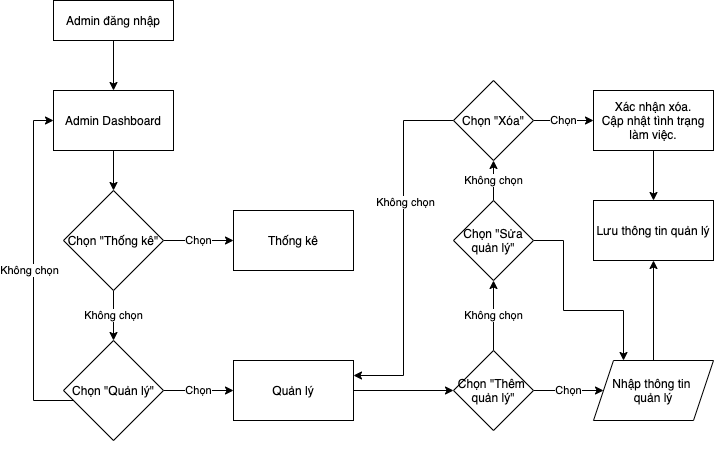
\includegraphics[scale = 0.6]{GCF Charts/GCF_Admin.png}
			\caption{Luồng điều khiển của Admin}
		\end{center}
	\end{figure}
	
	\begin{figure}[H]
		\begin{center}
			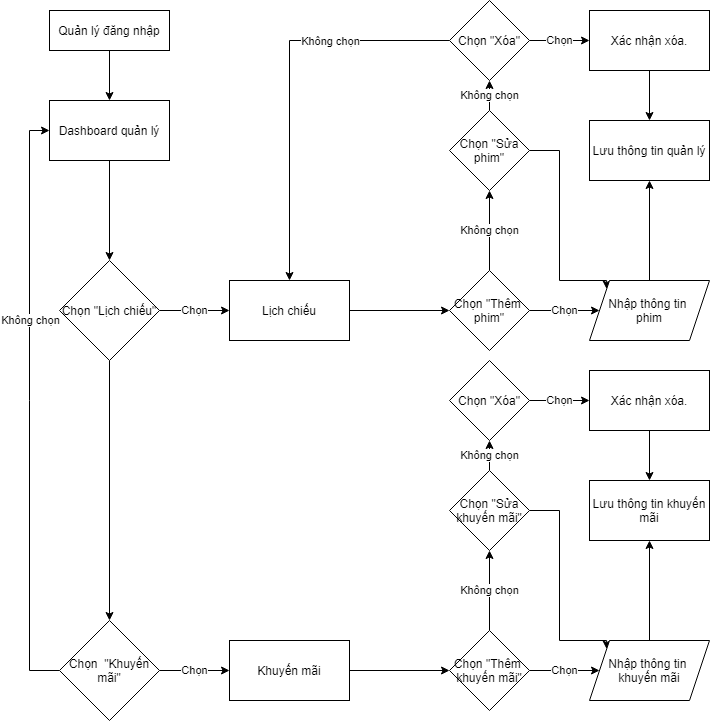
\includegraphics[scale = 0.6]{GCF Charts/GCF_Manager.png}
			\caption{Luồng điều khiển của Quản lý}
		\end{center}
	\end{figure}
	
	\begin{figure}[H]
		\begin{center}
			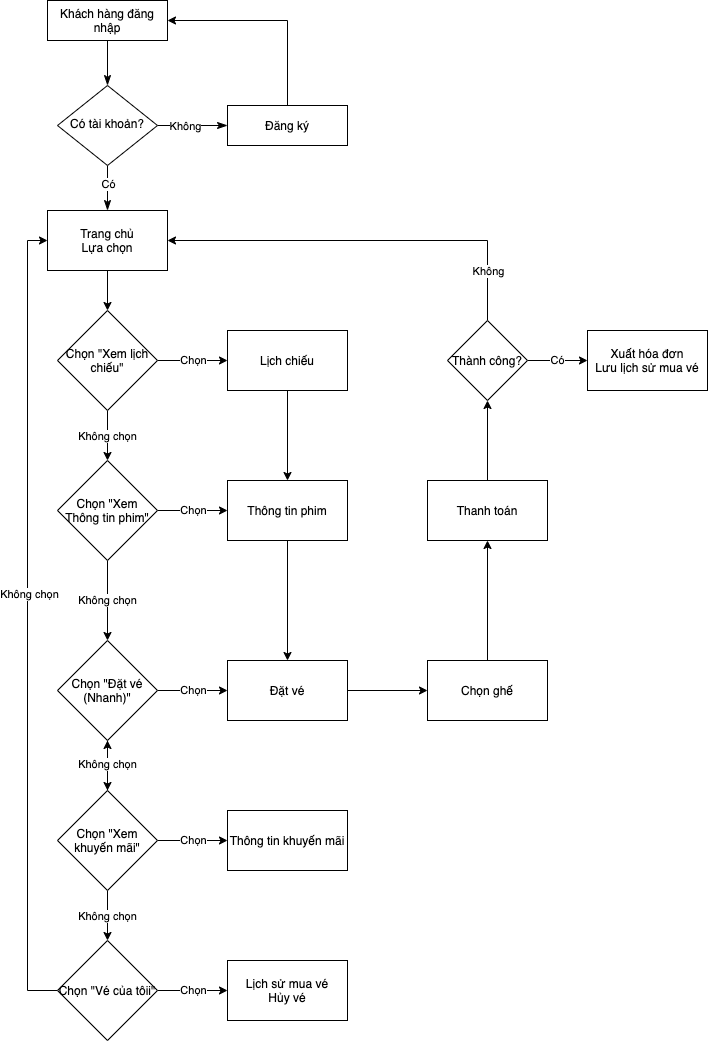
\includegraphics[scale = 0.6]{GCF Charts/GCF_User.png}
			\caption{Luồng điều khiển của Khách hàng}
		\end{center}
	\end{figure}
	
	
	\clearpage
	
	\subsection{Yêu cầu phần cứng}
	%Text description
	Phía client: Một máy tính cá nhân, tablet, điện thoại thông minh bất kì có thể sử dụng các trình duyệt web như Google Chrome, Microsoft Edge, Mozilla Firefox, Safari...
	\newline Phía server: Máy chủ vật lý hoặc máy chủ ảo có cấu hình tương đương tối thiểu như sau
	\begin{itemize}
		\item CPU: Intel Xeon 2.0 GHz, 2M Cache
		\item RAM: 2GB DDR4
		\item Lưu trữ: 240GB HDD/SSD
		\item Mạng: 100MBps cho cả Upload và Download, không giới hạn băng thông
	\end{itemize}
	
	\clearpage
	
	\section{Biểu đồ lớp}
	
	\subsection{Biểu đồ lớp}
	
	\subsection{Đặc tả các lớp}
	
	\subsubsection{Đặc tả lớp C1}
	
	\subsubsection{Đặc tả lớp C2}
	
	\subsubsection{Đặc tả lớp C3}
	
	\clearpage
	
	\section{Thuật toán và cấu trúc dữ liệu}
	
	\subsection{Các thuật toán}
	
	\subsection{Các cấu trúc dữ liệu}
>>>>>>> 6f25817f58bb95df29c448886101e0f5b313c456
	Ở hệ thống này không sử dụng các cấu trúc dữ liêu phức tạp
	
	
	\clearpage
	
	\section{Quản trị dự án và kế hoạch làm việc}
	
	\subsection{Tổng hợp đóng góp từ các thành viên của nhóm}
	
	\subsection{Báo cáo tiến độ và điều phối dự á}
	
	\subsection{Kế hoạch thực hiện}
	
	\subsection{Phân rã trách nhiệm (Breakdown of Responsibilities)}
	
	\clearpage
	
	\section{Tham khảo}
	\clearpage
	
\end{document}